%%\documentclass[sigconf]{acmart}
\documentclass[10pt,twocolumn]{article}

\title{Binge: Processing All of the Things with a BINary-at-the-EdGe}
\author{
        Kevin M. Greenan\\
        BRB Inc.\\
        Santa Cruz, CA 950602
}
\date{\today}


\usepackage{pdfpages}
\usepackage{listings}
\usepackage{listings-golang}
\usepackage{makecell}

\renewcommand\theadalign{bc}
\renewcommand\theadfont{\bfseries}
\renewcommand\theadgape{\Gape[4pt]}
\renewcommand\cellgape{\Gape[4pt]}

\lstset{basicstyle=\small\ttfamily,columns=fullflexible,language=Golang}
\begin{document}
\maketitle

\begin{abstract}
Most stream and event processing is done using popular Stream Processing
Engines (SPE), such as Apache Storm, using event-based design patterns within a
custom application stack, or a combination of the two.  In either case, the
foundation of these architectures relies on a centralized event bus or pub/sub
system that acts as a buffer for processing events.  While this approach is
well understood and ubiquitous, it is not well-suited to many current and
future applications within edge computing and modern SaaS applications.  While
there will likely always be a need for centralized event buses and custom
application stacks, a great deal of stream processing can be done without an
SPE or core application stack.

In this paper, we present Binge (binary-at-the-edge), a lightweight, durable,
scalable, stream processing daemon that can run on commodity hardware without
the need for complex application and infrastructure configurations.  Each binge
instance only relies on its own local configuration, which allows it to scale
horizontally and heterogeneously.  We show that binge can be leveraged for
simple stream processing tasks at the IoT edge, VPC edge, PoP edge and as a
mesh of coordinating endpoints.
\end{abstract}


\section{Introduction}
The ubiquity of software-as-a-service (SaaS) (e.g., Salesforce, Slack, GitHub,
etc.) and cloud platform services (PaaS) (e.g., AWS, Google Cloud and Azure)
has created a complex ecosystem of integration platforms that integrate SaaS
services via events and APIs.  There are a great deal of products aimed at
automating decision making, tracking customer experience, automating
engineering processes, and so on.   These products are effectively consuming
event data from SaaS services and  processing it in managed PaaS services.
Integrating with a SaaS platform typically means subscribing to events,
consuming events and calling their APIs.  A basic integration platform may
consume all events from any number of SaaS integrations and publish them to
Kafka topics to be consumed by SPEs, custom microservice applications or big
data systems such as BigQuery.  

The many emerging IoT use cases are very similar.  That is, consuming disperate
events, publishing them to a centralized event bus and using SPEs to process.
The main difference between the IoT use cases and the integration platform use
case is the definition of edge.  In the case of IoT, the edge is as close to
the devices as possible, while the integration platform is usually a
point-of-presence (PoP) or a load balancer in the platform's VPC or data
center.   In each case, there are different assumptions around what resources
are available.  For example, it might not be safe to assume now-latency access
to a Kafka broker in the IoT use case, but the integration platform edge may be
on the same network as a Kafka cluster.  In the most ideal case, all filtering,
transformation and processing can be done as close to the edge as possible.  In
reality, most of this is still done in a centralized fashion, albeit in
distributed SPEs and microservice architectures.

The goal of binge is to simplify moving as much event processing as possible to
the edge (depending on what edge means for the application) in a way that is
durable, flexible and easy to operate.  The goal is not to usurp existing SPEs
or event based architectures, but to compliment them in a way that performs
processing in the most appropriate tier (edge vs. hub) depending on cost,
resources, performance, etc.

\section{Outline}
The remainder of this article is organized as follows.
Sections~\ref{binge:design}~and~\ref{binge:implementation} cover the design and
implementation of Binge.  We go through a few potential use cases for using
Binge in Section~\ref{usecases}.  We evaluate the performance of Binge in
Section~\ref{evaluation}.  Section~\ref{previous:work} gives account of
previous work.  Finally, Section~\ref{future:work} covers future work and we
conclude in Section~\ref{conclusions}.

\section{Binge Design}\label{binge:design}

The high-level components of Binge are illustrated in
Figure~\ref{fig:binge-daemon}.  Opposed to most SPEs and microservice
architectures, which require a great deal of configuration and moving parts,
Binge is composed of a single binary that can run as a  command (e.g.
process a single event in a Lmabda for use in a serverless architecture, for
testing or debugging) or as a daemon.  The figure shows the components used for
daemon mode.  Binge exposes a HTTP endpoint that accepts POST requests
containing JSON-formatted content, each representing an event.  All events
consumed by the daemon are persisted to a durable queue, which are consumed by
workers.  Each event will be processed by a worker in one or more pipelines
defined in the configuration.  Once a worker has completed processing an event,
it will ack the event and pick up more work.  This in combination with
checkpointing (discussed later) allows the each daemon to be killed without
losing events or processing state.  Later we will discuss tradeoffs with the
various durability configurations. 

\begin{figure}[h]
\centering
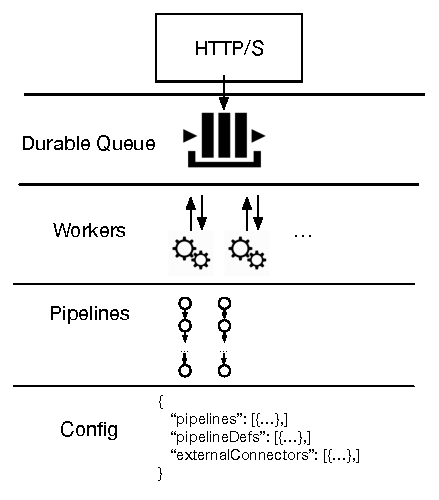
\includegraphics[scale=0.60]{figures/binge-daemon.pdf}
\caption{This}
\label{fig:binge-daemon}
\end{figure}

Today, the daemon can be also be configured in stateless mode, which disables
the durable queue.  This configuration can be used in cases where reliable
delivery is less important than performance.  In addition, there are some use
cases where HTTP is not a sufficient interface.  Adding new endpoint interfaces
is relatively easy.  For example, we can create a consumer interface that
consumes messages from MTTQ queues when running in an IoT edge.  The only
difference here is that the daemon operates in a pull model opposed to the push
model of an HTTP endpoint.

The rest of this section will be devoted to digging deeper into the durable
queueing mechanism, pipelines, configuration and tradeoffs between different
configurations.

\subsection{Durable Queue}

All events posted to the binge daemon are immediately placed into a durable
queue before replying with success to the caller.  This is done for two
reasons.  First, it allows this or another daemon to process events that were
either unprocessed or in-flight after a crash.  Second, it provides a buffering
mechanism between the incoming events and the workers, preventing the need to
apply backpressure.  The remainer of this section is devoted to both of these
aspects of the durable queue.

\subsubsection{Event Processing and Crashes}

The durable queue maintains three buckets: in-flight, unprocessed and an
internal bucket for queue metadata, such as head and tail location of the
unprocessed events.  Figure~\ref{fig:durable-queue} shows the basic data
structures and a simple example.  The queue can technically be backed by any
underlying data structure that implements the following interface:

\begin{lstlisting}[linewidth=\columnwidth,breaklines=true]
type DQueue interface {
    Dequeue() (*QueueItem, error)
    Enqueue(v []byte) error
    Ack(*QueueItem) error
}
\end{lstlisting}

We currently rely on BoltDB (https://github.com/etcd-io/bbolt) for persistence.
Swapping out backends is trivial as long as the backing system can be mapped to
a Key-Value interface.  We chose BoltDB because it is fast, stable and runs
in-process, which allows us to minimize the number of external dependencies.
Running BoltDB also allows for configurations to easily leverage external block
stores for persistence, which lends itself to more ephemeral environments.

As shown in Figure~\ref{fig:durable-queue}, we have $5$ unprocessed events a
$0$ in-flight, before a worker pulls an event off the queue.  Prior to
returning the event to the worker, $Evt_{3}$ is atomically swapped to the
in-flight queue.  An event is not removed from the in-flight queue until it is
acked.  While processing the event, the daemon (as well as the worker) crashes
and restarts.  Before accespting any new connections the daemon will process
the unprocessed and in-flight queues.  Depending on the current status of each
event, some may remain on the in-flight queue after the start-up process
finishes.  This could be due to an external resource being unavailable or an
issue with the state of the event or checkpoint.  The proper action depends
mostly on the use case and could be a combination of: throw the events away,
fire an alert, or forward the events to another system \footnote{ToDo: Add
recovery rules to the pipelines.  For example, add an OnFail section to a
process, which can take an action when it fails}

\begin{figure}[h]
\centering
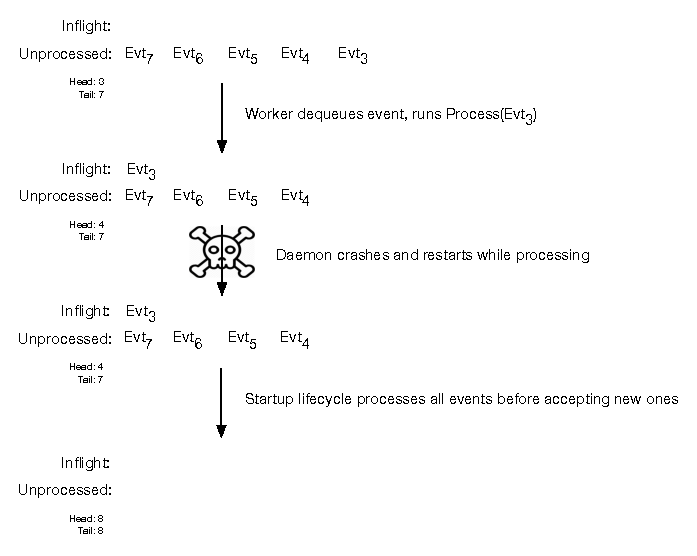
\includegraphics[scale=0.60]{figures/durable-queue.pdf}
\caption{This}
\label{fig:durable-queue}
\end{figure}

The self-contained nature of binge also allows many instances to serve the same
event streams where daemons fail and recover without direct coordination.  For
example, if running in Kubernetes, a binge pod can be bounced and will simply
continue using the same persistent volume when it restarts.  We get similar
behavior when running in VMs or on physical hardware, provided a supervisor
detects the daemon stopped and requires restart.

\subsubsection{Backpressure}

We want to ensure all events are eventually processed, but there are times when
a daemon gets overloaded and applies backpressure, usually in the form of a
HTTP $429$ response.  One way to avoid the need to apply backpressure is to put
a buffer between the enpoint serving the request and the processing.  Here, the
tradeoff is that returning a $200$ OK only means the event has been persisted
and the event is hopefully processed.  As we have shown, we use a durable queue
as our buffer.  We use tracing to ensure we have visibility into the state of
all events.  

Given that binge may be running in a resource constrained environment, it is
possible that a daemon is overloaded and the queue exhausts disk space in
either a local or remote volume.  There are two complimentary ways to ensure
events are not lost: spin-up more instances (if possible) and/or specify
high-water marks used to offload the latest events to an external system until
a low-water mark is hit and we can pull those events in \footnote{ToDo: This
can be worked into the configuration, likely as a command line option for the
daemon}.

In the worst case, the daemon is running in a resource constrained environment,
runs out of disk space and eventually has to resort to backpressure.  In any
case, the daemon itself can be configured to mitigate this issue by offloading
newly consumed events until a low-water mark is hit.

\subsubsection{Stateless Mode}

As previously discussed, binge can run in stateless mode, either as a daemon or
in command mode.  Stateless mode effectively disables the durable queueing
mechanism and crash recovery lifecycle.  This means that backpressure will be
applied when the all of the daemon threads or allowable connections are
consumed, and unprocessed events will likely be dropped in the event of a
crash.  

This mode is best suited for cases where the source events can be safely
dropped or binge is run within a serverless architecture (i.e. command
mode).  As we will show in the next section, pipelines provide a checkpoint
mechanism that can ensure indivdual pipeline executions can proceed after a
crash.

\subsection{Pipeline Processes}\label{sec:pipelineproc}

Pipelines are at the heart of binge.  Each event will be proceessed through
every pipeline configured for the daemon.  This allows different
binge/configuration artifacts to be deployed for specific events.  For example,
you can deploy a specific configuration to an auto-scale group to serve events
for your CI/CD processes from GitHub, GitLab and CircleCI, while a separate
configuration is deployed to an auto-scale group to serve your Slack
events.

A pipeline is a colleciton of processes that are applied in sequetial order.
Each process must implement the following interface to be used within a pipeline:

\begin{lstlisting}[linewidth=\columnwidth,breaklines=true]
type PipelineProcess interface {
	Process(ctx context.Context, in map[string]interface{}) (map[string]interface{}, error)
}
\end{lstlisting}

The context is used to plumb contextual information through the pipeline, the
individual processes and onto external dependencies, such as Key-Value Stores.
As we will see the pipelines can be configured to automatically add
OpenTelemetry~\cite{OT} trace context to select requests.

At a high level, the Process function takes in a map and outputs a map.  The
source can be any structured data format that can be converted into a map, such
as JSON, YAML, CSV, protobuf, etc.  As we will see, this simple abstraction
allows one to define a rich set of operations that can handle many stream
processing tasks.

Each pipeline invocation will process an event serially through the pipeline.
We rely on a $Completable$/$Future$ abstraction, which simplifies asynchronous
processing.  Since Golang does not have native support for $Futures$, we
created our own implementation.  In a nutshell, a $Completable$ contains the
eventual result of a computation, which is exposed to the caller as a $Future$.
The caller can invoke $Future.Get()$ to block and obtain the result, or rely on
callbacks to perform actions on the result.  To enable highly concurrent
pipelines, the Future abstraction exposes a $Then(Runnable)$ function
that will run the provided runnable using output of the parent future as input,
when the parent future completes.  This model maps very nicely with invoking
pipelines on events.

\begin{figure}
\begin{lstlisting}[linewidth=\columnwidth,breaklines=true]
// RunnableStartProcess will create a runnable that calls 
// outMap = pipelineProcess1.Process(inMap)
runnable1 := NewRunnableStartProcess(pipelineProcess1, inMap)

// RunnablePartialProcess will create a runnable that implements 
// SetInData(x map[string]interface{}) and runs pipelineProcess2.Process(SetInData(x))
runnable2 := NewRunnablePartialProcess(pipelineProcess2)
runnable3 := NewRunnablePartialProcess(pipelineProcess3)

// A pipeline invocation is a chain of futures
f1 := CreateFuture(runnable1)
f2 := f1.Then(runnable2)
f3 := f2.Then(runnable3)
f3.Get()
\end{lstlisting}
\caption{Example of chaining runnables}
\label{fig:runnables}
\end{figure}

Figure~\ref{fig:runnables} illustrates how the Future abstraction fits nicely
with pipeline invocation.  Each pipeline process is contained in a runnable
object.  A $RunnableStartProcess$ must implement $Run()$, which will simply
invoke $Process$.  A $RunnablePartialProcess$ must implement both $Run$ and
$SetInData$, where $SetInData$ is called by $Then$ with the result of the
previous future and $Run$ invokes $Process$ with the result.

In addition to chaining, callbacks such as Prepare, OnSuccess and OnFailure are
used to add instrumentation (meters and counters) and trace information (spans)
to the individual processes.

\subsection{Pipeline Configuration}

There are five manjor components to a pipeline configuration:

\begin{itemize}
\item{{\bfseries External Systems:}} This contains global configuration for external systems, such as databases, key-value stores, SPEs, HTTP/gRPC endpoints or pub/sub systems.
\item{{\bfseries Pipeline Process Definition:}} This contains the configuration for a pipeline process that can be referenced by one or more pieplines.
\item{{\bfseries Pipeline Manifests:}} Each pipeline will contain a manifest, which is a list of ordered pipeline processes that define the pipeline.
\item{{\bfseries Checkpoint Process:}} The checkpoint process is a special process that will checkpoint state to a provided external system.  It is configured per pipeline.
\item{{\bfseries Pipelines:}} Pipelines is root configuration object for binge and contains the external systems, pipeline process definitions and pipeline manifests.
\end{itemize}

\subsection{Pipeline Process Types}

\begin{table*}[t]
\centering
\begin{tabular}{|c|c|c|c|c|}
\hline
{\bfseries Type} & {\bfseries Desc} & {\bfseries Cond?} & {\bfseries Update?} & {\bfseries Stateful?} \\ \hline
Annotator & Add annotations to output map & Yes & Yes & No \\ \hline
Aggregator & Update an aggregation based on one or more fields & Yes & Yes & Yes \\ \hline
Completor & \makecell{Define a join on $N$ fields and emit a completion \\ annotation when a specific value for all $N$ fields is observed} & No & Yes & Yes \\ \hline
Filter & Filter (or inverse filter) fields using string match or regex & No & Yes & No \\ \hline
Spawner & Spawn a job & Yes & No & No \\ \hline
Transformer & Transform one or more fields of the source map & Yes & Yes & No \\ \hline
Tee & Send the current map or a transformed map to an external system & Yes & No & No \\ \hline
\end{tabular}
\caption{Process types}
\label{tab:processtypes}
\end{table*}

As shown in Table~\ref{tab:processtypes}, there are seven process types.  As
described in Section~\ref{sec:pipelineproc}, a process essentially processes an
input map and returns an output map.  Many of the processes can be
conditionally guarded with a condition implementing the folloowing interface:

\begin{lstlisting}[linewidth=\columnwidth,breaklines=true]
type Condition interface {
    Evaluate(in map[string]interface{}) (bool, error)
}
\end{lstlisting}

A condition is applied to the input map, where the target process will run if
and only if Condition evaluates to true.  An error will either lead to failure of
the pipeline run for this event or will invoke the error handler specified in the
process definition.

All but two of the processes apply updates to the map.  Note that the input map
left untouched and an update simply means the output map is a transformed copy
of the input map.

The Annotator, Filter and Spawner are the simplest of the processes, and all
can be defined with a conditional guard.  An Annotator will simply add
annotations to the map.  A Filter will either apply a filter or inverse filter
to a map.  Finally, a Spawner will spawn a job.  Currently, jobs are processes
that are spawned locally must adhere to the same interface a Processes.  That
is, a JSON-encoded map is written to standard input and a JSON-encoded map is
expected on standard output.

The remaining processes require more explanation and we will spend the rest of
this section describing them with a few examples.

\subsection{Aggregator}

An Aggregator exposees many common aggregations provided by SPEs and databases.  Currently,
we support Sum, Max, Min, Avg, Count and Histograms.  An Aggregator is defined by 4 components:

\begin{itemize}
\item{{\bfseries State Store}} This specifies the external system used to store
the aggregation, which can be anything from a local file system to an external
key-value store.
\item{{\bfseries Field Key}} This is the field key that corresponds to the value to aggregate.
\item{{\bfseries Aggregation Type}} This is the type of aggregatioon to apply.
\item{{\bfseries Group By}} Group by applies to all but the Histogram aggregation and will aggregate by the keys provided.
\end{itemize}

Figure~\ref{fig:aggregation} shows an example snapshot of a pipeline run
containing three aggregation processes.  First, we see the output map of the
previous process passed into the Sum aggregation.  The Aggregator process will
try to fetch state for this aggregation.  If there is no state, it will create
new state.  In either case, a new annotation is added to the map containing the
current state of the aggregation after it is updated.  These annotations can be
used by downstream processes to conditionally run processes, to further
aggregate or make other decisions.  The figure also illustrates the use of
histogram aggregations and a simple count.

This example also highlights another well-known issue with stateful stream
processes: tracking consistent state.  There are three main tradeoffs that arise
with respect to stateful processes:

\begin{itemize}
\item{{\bfseries Consistency}} Maintaining consistent state requires coordination or centralization.
\item{{\bfseries Performance}} Requiring consistent stateful processes will negatively impact latency.
\item{{\bfseries Starvation}} Requiring consistent stateful processes could lead to starvation.
\end{itemize}

There are two modes of operation here:

\begin{itemize}
\item{Use a centralized key-value store to maintain state.  At minimum we would
want atomic put and delete to ensure consistency.}
\item{Rely on a local persistent store (file system or local key-vallue store)
and aggregate the aggregations at a binge sink that is close to a centralized
key-value store.}
\end{itemize}

The first option is the easiest to reason about, since we simply specify an
external system to use.  The major cloud providers have a variety of options
that can be deployed at the push of a button.  Here, the conceern is
performance: increase in latency due to round-trip time and contention.
Contention could be mitigated using higih-performance key-value stores, such as
Anna~\cite{ANNA}.  In either case, the distance between the binge process and
the centralized key-value store will largely dictate the performance overhead.

The second option relies on the existance of a binge-mesh, where a pipeline
maintains local aggregation state and relies on a downstream binge process to
perform the final aggregation.  In this case, the final aggregation could be
performed closer to a centralized key-value store.  Note that here the
round-trip time doesn't change, but our throughput will likely be higher than
the first option.  The main disadvatage to this approach is managing the mesh
of binge processes.  We will cover this in Section~\ref{sec:orchestration}.

\begin{figure*}
\centering
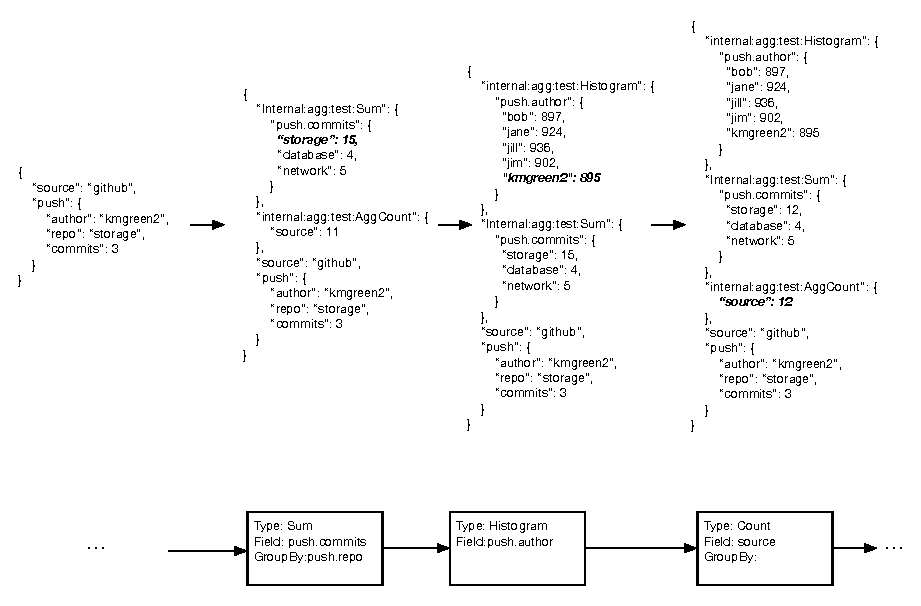
\includegraphics{figures/aggregation.pdf}
\caption{Figure}
\label{fig:aggregation}
\end{figure*}


\section{Binge Implementaion}\label{binge:implementation}
\section{Orchestration}\label{sec:orchestration}
\section{Example Use Cases}\label{usecases}
\section{Performance Evaluation}\label{evaluation}
\section{Previous work}\label{previous:work}
\section{Limitations and Future Work}\label{future:work}
\section{Conclusions}\label{conclusions}
We worked hard, and achieved very little.

\bibliographystyle{abbrv}
\bibliography{main}

\end{document}
This is never printed
